%% LyX 2.1.4 created this file.  For more info, see http://www.lyx.org/.
%% Do not edit unless you really know what you are doing.
\documentclass[11pt,czech,american]{book}
\usepackage[T1]{fontenc}
\usepackage[utf8]{inputenc}
\usepackage[a4paper]{geometry}
\geometry{verbose,tmargin=4cm,bmargin=3cm,lmargin=3cm,rmargin=2cm,headheight=0.8cm,headsep=1cm,footskip=0.5cm}
\pagestyle{headings}
\setcounter{secnumdepth}{3}
\usepackage{url}
\usepackage{amsmath}
\usepackage{mathtools}
\usepackage{amsthm}
\usepackage{amssymb}
\usepackage{amstext}
\usepackage{graphicx}
\usepackage{setspace}
\usepackage{wrapfig}
\usepackage{algorithm}
\usepackage{algpseudocode}
\usepackage{svg}
\usepackage{outlines}
\usepackage[normalem]{ulem}
\usepackage{dirtytalk}
% \usepackage{subcaption}
% \usepackage{subfigure}

\makeatletter
\newenvironment{lyxlist}[1]
{\begin{list}{}
{\settowidth{\labelwidth}{#1}
 \setlength{\leftmargin}{\labelwidth}
 \addtolength{\leftmargin}{\labelsep}
 \renewcommand{\makelabel}[1]{##1\hfil}}}
{\end{list}}

\usepackage[varg]{txfonts}

\usepackage{indentfirst}

\clubpenalty=9500

\widowpenalty=9500

\hyphenation{CDFA HARDI HiPPIES IKEM InterTrack MEGIDDO MIMD MPFA DICOM ASCLEPIOS MedInria}

\renewcommand{\vec}[1]{\boldsymbol{#1}}
\newcommand{\code}{\texttt}

\newtheorem{thm}{Theorem} % [section]
\newtheorem{lem}{Lemma}
\newtheorem{prop}{Proposition}
\newtheorem{cor}{Corollary}
\newtheorem{conj}{Conjecture}
\newtheorem{dfn}{Definition}

\DeclareMathOperator{\id}{id}
\DeclareMathOperator*{\argmax}{arg\,max}
\DeclareMathOperator*{\argmin}{arg\,min}

% \DeclarePairedDelimiter\ceil{\lceil}{\rceil}
% \DeclarePairedDelimiter\floor{\lfloor}{\rfloor}

\def\code#1{\texttt{#1}}

\newcommand{\bd}[1]{\mathbf{#1}}
\newcommand{\RR}{\mathbb{R}}      
\newcommand{\ZZ}{\mathbb{Z}}
\newcommand{\ZZP}{\mathbb{Z}+^}
\newcommand{\NN}{\mathbb{N}}
\newcommand{\QQ}{\mathbb{Q}}
\newcommand{\CC}{\mathbb{C}}
\newcommand{\col}[1]{\left[\begin{matrix} #1 \end{matrix} \right]}
\newcommand{\comb}[2]{\binom{#1^2 + #2^2}{#1+#2}}
\newcommand{\Tau}{\mathrm{T}}

\DeclarePairedDelimiter\norm{\lVert}{\rVert}
\interfootnotelinepenalty=10000 % ! THIS MAY CAUSE TROUBLE !

\makeatother

\usepackage{babel}
\begin{document}

\def\documentdate{\today}

\pagestyle{empty}


\noindent \begin{center}
\begin{minipage}[c]{3cm}%
\noindent \begin{center}
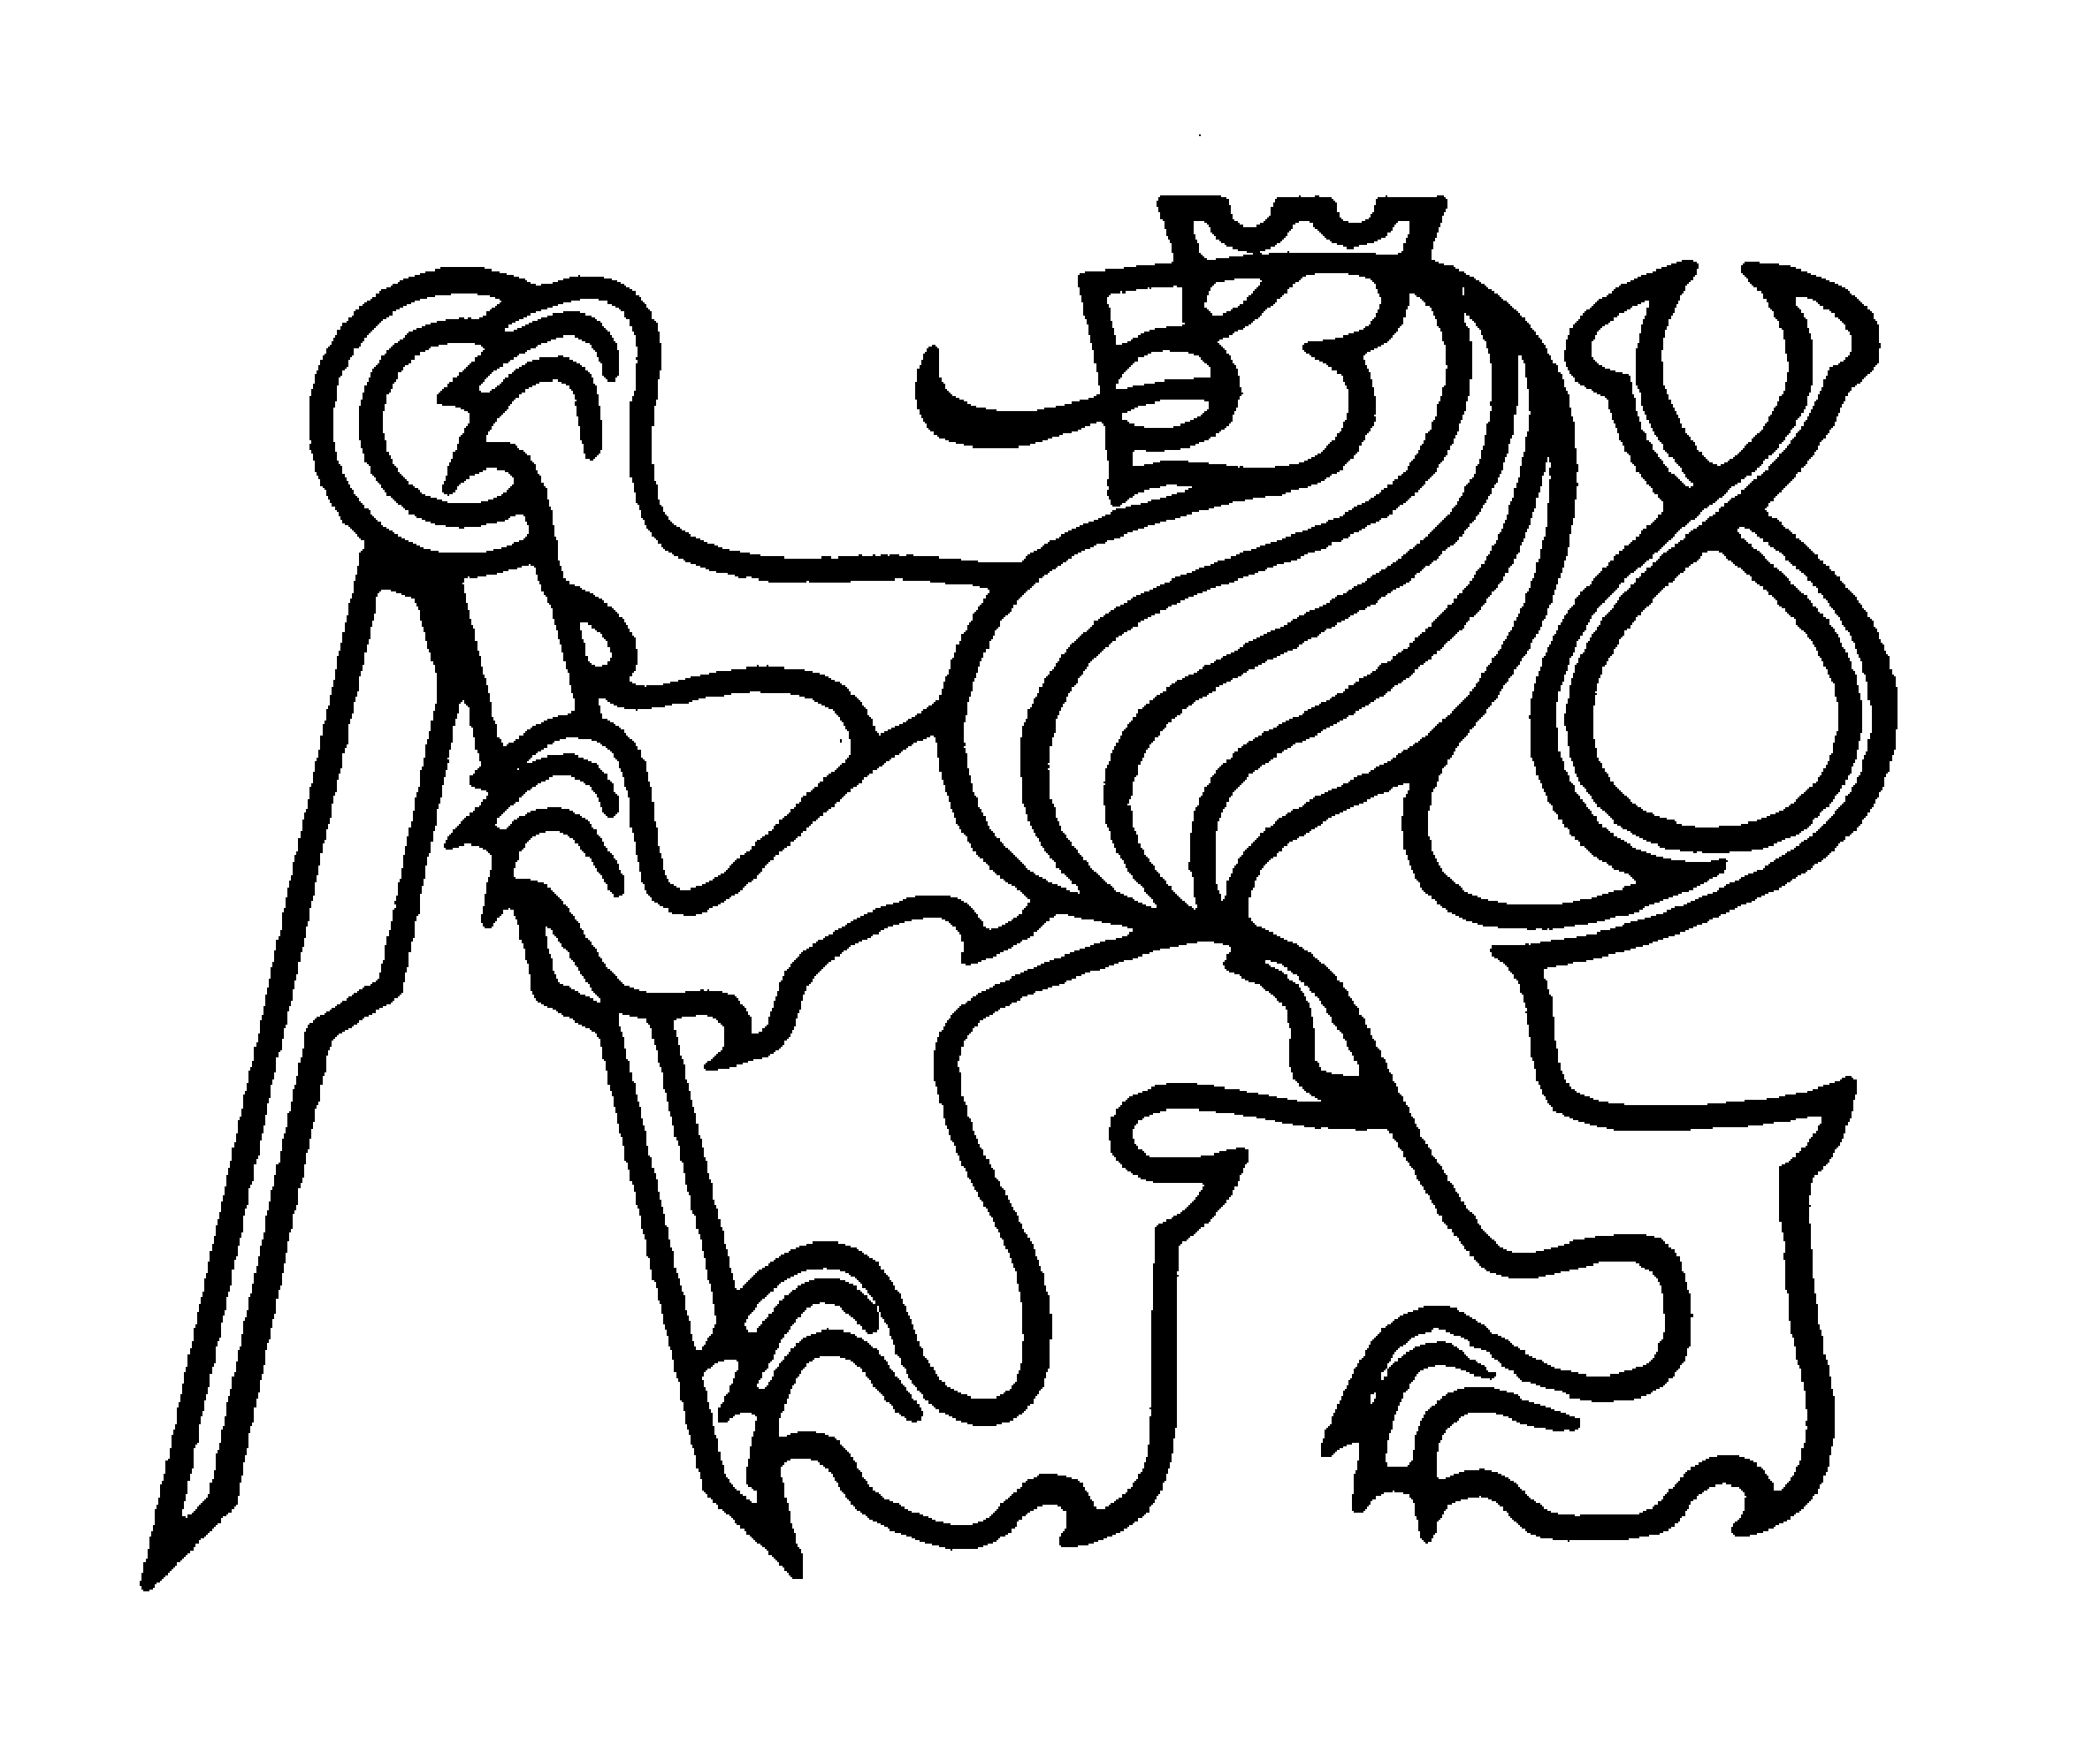
\includegraphics[width=3cm,height=3cm,keepaspectratio]{Images/TITLE/cvut}
\par\end{center}%
\end{minipage}%
\begin{minipage}[c]{0.6\linewidth}%
\begin{center}
\textsc{\large{}Czech Technical University in Prague}{\large{}}\\
{\large{}Faculty of Nuclear Sciences and Physical Engineering}
\par\end{center}%
\end{minipage}%
\begin{minipage}[c]{3cm}%
\noindent \begin{center}

\includegraphics[width=3cm,height=3cm,keepaspectratio]{Images/TITLE/fjfi}
\par\end{center}%
\end{minipage}
\par\end{center}

\vspace{3cm}


\begin{center}
  \textbf{\huge{}Biomarker Analysis of Psychiatric Patients using EEG Signal Analysis and Machine Learning}
\par\end{center}{\huge \par}

\vspace{1cm}


\selectlanguage{czech}%
\begin{center}
\textbf{\huge{}Analýza biomarkerů psychiatrických pacientů pomocí analýzy EEG signálu a strojového učení}
\par\end{center}{\huge \par}

\selectlanguage{american}%
\vspace{2cm}


\begin{center}
{\large{}Diploma thesis}
\par\end{center}{\large \par}

\vfill{}

\begin{lyxlist}{MMMMMMMMM}
\begin{singlespace}
\item [{Author:}] \textbf{Miroslav Kovář}
\item [{Supervisor:}] \textbf{M.Sc. M.A. Sebastián Basterrech, Ph.D.}
\end{singlespace}

% \item [{Language~advisor:}] \textbf{Mgr. Jméno Učitelky Angličtiny}
\begin{singlespace}
\item [{Academic~year:}]2018/2019\end{singlespace}

\end{lyxlist}
\newpage{}

~\newpage{}

~

\vfill{}


\begin{center}
- Zadání práce -
\par\end{center}

\vfill{}


~\newpage{}

~

\vfill{}


\begin{center}
- Zadání práce (zadní strana) -
\par\end{center}

\vfill{}


~\newpage{}

\noindent \emph{\Large{}Acknowledgment:}{\Large \par}

\noindent Some acknoledgment here.

\vfill

\noindent \emph{\Large{}Author's declaration:}{\Large \par}

\noindent I declare that this research project is entirely
my own work and I have listed all the used sources in the bibliography.

\bigskip{}


\noindent Prague, \documentdate\hfill{}Miroslav Kovář

\vspace{2cm}


\newpage{}

~\newpage{}

\selectlanguage{czech}%
\begin{onehalfspace}
\noindent \emph{Název práce:}

\noindent \textbf{Analýza biomarkerů psychiatrických pacientů pomocí analýzy EEG signálu a strojového učení}
\end{onehalfspace}

\bigskip{}


\noindent \emph{Autor:} Miroslav Kovář

\bigskip{}


\noindent \emph{Obor:} Aplikace přírodních věd \bigskip{}


\noindent \emph{Zaměření:} Matematická informatika

\bigskip{}


\noindent \emph{Druh práce:} Diplomová práce

\bigskip{}


\noindent \emph{Vedoucí práce:} M.Sc. M.A. Sebastián Basterrech, Ph.D.,
Artificial Intelligence Center, FEE, CTU Prague

\bigskip{}


% \noindent \emph{Konzultant:} doc. RNDr. Jméno Konzultanta, CSc., pracoviště
% konzultanta. Pouze pokud konzultant byl jmenován.

\bigskip{}


\noindent \emph{Abstrakt:} \bigskip{}


\noindent \emph{Klíčová slova:} 

\selectlanguage{american}%
\vfill{}
~

\begin{onehalfspace}
\noindent \emph{Title:}

\noindent \textbf{Biomarker Analysis of Psychiatric Patients using EEG Signal Analysis and Machine Learning}
\end{onehalfspace}

\bigskip{}


\noindent \emph{Author:} Miroslav Kovář

\bigskip{}


\noindent \emph{Abstract:} 

\bigskip{}


\noindent \emph{Key words:} 

%keywords in alphabetical order separated by commas

\newpage{}

~\newpage{}

\pagestyle{plain}

\tableofcontents{}

\newpage{}


\chapter*{Introduction}
Depression is one of the most common brain disorders - it affacts 121-300 million people worldwide, and this number is expected to increase in the future \cite{rodriguez2015} \cite{whodepression}. Although effective treatments are known, World Health Organization estimates that fewer than half of those affected receive those treatments. Major barriers include insufficient resources, lack of properly trained practitioners, inaccurate assessment and misdiagnosis. \cite{whodepression} 

For these reasons, it is important that affordable, fast, accurate, and easy to use methods for its diagnosis are developed. Although electroencephalography (EEG) \footnote{In this work, we will use the same abreviation for electroencephalography (recording method) and electroencephalographam (the recorded data) where the distinction is apparent from the context.} may be one such method thanks to its comparatively low-cost and easy recording process, comparatively little research has been focused on this area. Non-linear dynamical analysis in particular has been proven very effective at diagnosing mental disorders, and this work is aimed at contributing to this important and relatively new topic.

In \textbf{Chapter 1}, we present some of the classical theory and methods of non-linear dynamical analysis and chaos theory, with focus on the terms used in the following text.

In \textbf{Chapter 2}, we introduce the basic concepts and terminology used in design and evaluation of convolutional neural networks.

In \textbf{Chapter 3}, we describe the methods proposed, experiments performed, and results obtained.

% \addcontentsline{toc}{chapter}{Introduction}

\chapter{Non-linear time series analysis}
The nature is constantly undergoing change. Around us, we can observe many processes evolving in time. Some of the aspects of these processes, we can measure, and attempt to discover apparent patterns in those measurements. The most simple of those patterns are periodicities, probably best exemplified, and first noticed by humans, are the motions of the sun and the moon. Weather, on the other hand, is an example of processes seemingly defying any simple description.

Those examples represent two classes of processes existent before the rise of non-linear dynamics: \cite{andreas2000}
\begin{description}
  \item[Deterministic process]: periodic (or quasi-periodic), fully describable by its Fourier spectrum.
  \item[Stochasitc process]: influenced by forces unpredictable under all circumstances.
\end{description}
Non-linear dynamical analysis studies a third class of processes, which are irregular, non-periodic, yet still deterministic. Every non-periodic, deterministic process is non-linear (bot not necessarily the other way around). Existence of these processes was known already in mid-19th century to J. C. Maxwell, but the field began to be developed only with the rising feasibility of numerical simulations, peaking in 1980s. \cite{andreas2000}

\section{EEG signal}
Electroencephalography (EEG) is a noninvasive method of measuring fluctuations of electric potentials near the skull caused by synchronized firing of neurons in the upper cortical layers. Electroencephalogram is a record of these fluctuations measured over a period of time. \cite{nunez2006}

Although EEG has significantly lower spatial resolution in comparison with other diagnostic techniques such as functional magnetic resonance sampling (fMRI) and magnetoencephalography (MEG) \cite{srinivasan1999} and enables measuring only neural activity near the cortical surface, as a depression diagnostic tool, it has numerous benefits. Importantly, its significantly lower costs \cite{vespa1999} \cite{hamalainen1993}, high portability, and ease of operation imply increased availability to the patients \cite{schultz2012}. Moreover, it is perfectly noninvasive, which means less complications such as claustrophopia or anxiety \cite{murphy1997}.

Although the science of EEG signal analysis as a diagnostic tool brings compelling clinical promise as a result of the aforementioned benefits, it also presents multiple technical and conceptual challenges. 

\begin{figure} 
\centering
\noindent\makebox[\textwidth]{%
  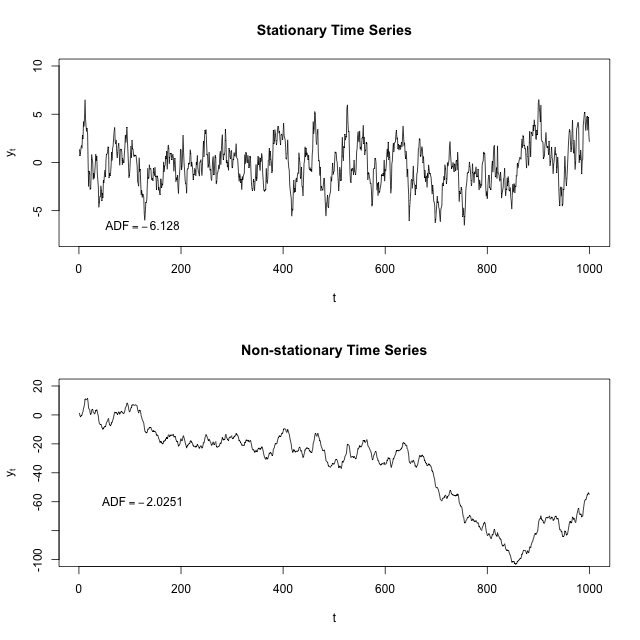
\includegraphics[width=0.8\textwidth]{Images/stationarycomparison.png} }
  \caption{A comparison of stationary and non-stationary time series. (Courtesy: Protonk)}
\label{fig:statnonstatcomp}

\end{figure}
\begin{dfn}[\cite{priestley1988}]
  A series $\{X_t\}_{t \in \ZZ}$ is called \textbf{stationary}, if $\{X_t\}_{t \in \ZZ}$ for any set of times $t_1, t_2, \dots, t_n$ and any $k \in \mathrm{N}$, $P[X_{t_1}, X_{t_2}, \dots, X_{t_n}] = P[X_{t_1+k}, X_{t_2+k}, \dots, X_{t_n+k}]$, i.e. the joint probability distribution of $\{X_t\}_{t \in \ZZ}$ is not a function of time. It is called \textbf{non-stationary}, if it is not stationary.
\end{dfn}

\begin{dfn}[\cite{bickel1996}]
   A series $\{X_t\}_{t \in \ZZ}$ is called (noisy chaotic) \textbf{non-linear}, if it satisfies the relation
   \begin{align}
     X_t = f(X_{t-1}) + \epsilon_t
   \end{align}
   for a general $f : \RR \rightarrow \RR$.
\end{dfn}

EEG signals are prone to be infected with \emph{noise} due to imperfect isolation from surrounding environment. They are known to be \emph{transient, non-Gaussian, non-stationary and nonlinear} \cite{kaplan2005} \cite{stam2005}. Since some patterns do not activate relative to a stimulus, a successful classifier must be able to detect a pattern \emph{regardless of its starting time}, or find one. And finally, EEG records are relatively high dimensional - 16 electrodes sampling at 256 Hz result 4096 data points par second.

Moreover, due to the phenomenon of neural oscillations, patterns may appear in multiple frequency bands, from slow cortical potentials of $\delta$-waves at 0.5-4 Hz, to high $\gamma$ frequency band at 70-150 Hz. 

Patterns of oscillatory activity in various frequency band have been linked to various mental states \cite{canolty2006} \cite{buzsaki2004} and diseases such as epilepsy \cite{shusterman2008}, tremor \cite{mcauley2000}, Parkinson's disease and depression \cite{llinas1999}. Many of the diseases, including depression, share common oscillatory patterns known as thalamocortical dysrythmia, characterized by descrease in normal resting-state $\alpha$ (8-12 Hz) activity slowing down to $\theta$ (4-8 Hz) frequencies, accompanied by increase in $\beta$ and $\gamma$ (25-50 Hz) activity. \cite{vanneste2018}

\section{Limitations in application to EEG}

Some authors suggests that the since most plausible research target for explaining the brain dynamics are the assemblies of coupled and synchronously active neurons, and since majority of those assemblies are describable by non-linear differential equations, principles derived from nonlinear dynamics are applicable to characterization of these neuronal systems. \cite{kaplan2005} 

The approach of estimating a finite embedding dimension, however, has been doubted by some of the most prominent figures in the field of non-linear dynamical analysis, such as the originators of Grassberger-Procaccia algorithm. There is very little evidence for the seemingly improbable hypothesis that such complex system with many extrinsic influences and interactions, such as the brain, would exhibit a level of comlexity comparable to e.g. a Lorenz system. Presumably, the the observed estimates of low dimension are due to artifacts or limited data size. \cite{grassberger1986climatic} \cite{procaccia1988complex}. However, as we will see in Section \ref{sec:applications}, the techniqes derived from these theories still provide some useful information and are successfully applied in many practical situations. Therefore, it seems to be the case that indeed, brain dynamics are much more complex than we are forced to assume based on the theory, but non-linear dynamical analysis still manages to capture some of its important aspects.

\section{Dynamical systems} \label{sec:dynamical-systems}

\begin{dfn}[\cite{andreas2000}]
  Assume that state of a system can be fully described by a finite set of $d$ variabes, such that each state corresponds to a point $\mathbf{x} \in M$, where $M$ is a $d$-dimensional differentiable manifold. Then we will call $M$ a (true) \textbf{state space} or, equivalently, a (true) \textbf{phase space}, and $d$ its (true) \textbf{dimension}.
\end{dfn}

Although in this study, we will only consider Euclidean $M$, the true state space is needs not necessarily be Euclidean. For example, if some of the state variables are angles, the state space exhibits toroidal topology. However, any topological manifold is locally Euclidean \cite{lee2010introduction} and, since, in EEG signal analysis both $M$ and $d$ are unknown, we have no alternative but to work in Euclidean $M$.

\begin{dfn}[\cite{andreas2000}]
  Let $\mathbf{x} \in \RR^m$ be an $d \in \NN$ dimensional state (phase) space vector dependent on time, and $\mathbf{F}$ a smooth vector field in $\RR^d$. A \textbf{deterministic dynamical system}\footnote{In this work, we are going to assume that brain is a deterministic dynamical system, and that any stochastic component is small and does not change non-linear properties of the system. Thus, by the term dynamical system, we will always mean a deterministic dynamical system.} is described by a set of $d$ differential equations
  \begin{align}
    \frac{d}{dt}\mathbf{x}(t) = \mathbf{F}(\mathbf{x}(t)), \qquad t \in \RR.
  \end{align}
\end{dfn}

In general, any system with temporally changing state is dynamic. A \emph{deterministic} dynamical system is describable by a model giving precise transition of a system from one state to another in time. This means that total description of system's evolution in its phase space (its \emph{trajectory}) is given by the initial state and a set of equations (if $\mathbf{F}$ satisfies certain reasonable properties). With \emph{stochastic} dynamical systems, such mapping is not possible, since these transitions are not given precisely.

A non-linear dynamical system is a system where the differential equations describing its dynamics are non-linear. Unlike in a linear system, changes in the initial state of a non-dynamical system are allowed to have a non-linear relationship to the state space trajectory of the system. \cite{kaplan2005}

It is important to note the obvious fact that in the case of EEG signal analysis, it is not possible to measure the true state of the system $\mathbf{x}(t)$. In fact, the observed variables are only a function of the true state of the system, $s(\mathbf{x}(t))$ for some (generally non-invertible) measurement function $s: \RR^d \rightarrow \RR^{d'}$, where $d' \ll d$. Morover, the time between subsequent measurements is limited by a sampling frequency and the values of the variables themselves are taken and stored with a limited precision.

(TODO: Add a few examples (Lorenz, Rossler, Mackey-Glass). Create my own plots instead of reusing.)

\section{Attractor}
Depending on the properties of $\mathbf{F}$, there are several possibilities of how the system might evolve when as $t \rightarrow \inf$. In the following, we will focus on dissipative dynamical systems.
\begin{dfn}[\cite{kantz2004}]
  A dynamical system is called dissipative, when it is the case that
  \begin{align}
    E[\mathrm{div} \mathbf{F}] < 0,
  \end{align}
  where the expectation is taken over the state space $M$. In other words, average state space volume of a set of initial conditions of non-zero measure is contracted as the system evolves. (TODO: How precise is this statement? Is it equivalent to the equation?)
\end{dfn}

For these systems, after sufficient passage of time, all future states will continue evolving on a bounded, time-invariant subset of $M$. This subset is a geometrical object called an \textbf{attractor}. Example of four basic attractors can be seen on Figure \ref{fig:attractors}.

\begin{figure} 
\centering
\noindent\makebox[\textwidth]{%
  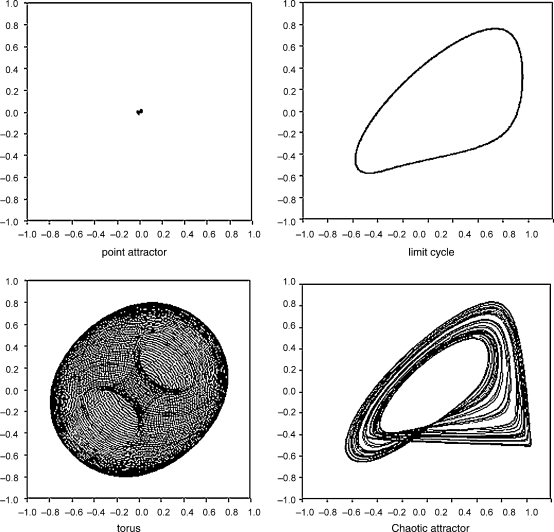
\includegraphics[width=0.8\textwidth]{Images/attractors.png} }
  \caption{Visualization of four common attractor types (units are arbitrary). Left to right, top to bottom:
    \emph{Point attractor} is the only type of attractor of linear deterministic dissipative systems. It consist of a single final state to which all points from the corresponding region of attraction evolve to.
    \emph{Limit cycle} corresponds to a periodic dynamical system. It is formed by set of states visited periodically, consituting a trajectory through the state space.
    \emph{Torus attractor} corresponds to a quasi-periodic dynamical system, resulting (in this example) from a superposition of two periodic oscillations.
    \emph{Chaotic} (strange) \emph{attractor}, characteristic of dynamical systems with extending (instead of shrinking) volumes in \emph{some} directions. Corresponding dynamical system may appear stochastic, yet still is completely deterministic. \cite{andreas2000} (\cite{stam2005})}
\label{fig:attractors}
\end{figure}

Since most physiogenerated signals are chaotic, their analysis is concerned primarily with \emph{chaotic} (strange) \emph{attractors}. These attractors are relatively complex, characteristic of dynamical systems with extending volumes in some directions. This property results fast divergence of two initial states, one of which has nonzero component in the direction of growth, i.e. sensitive dependence on the initial conditions. However, since atractors are bounded, the divergence eventually stops and the two trajectories fold together. This continuous expansion and folding may create an attractor with a \emph{fractal structure} (an example of a self-similar attractor is shown on Figure \ref{fig:self-similarity}). \cite{andreas2000} For our purposes it is sufficient to say that this means that these attractors can be characterized as having (quantifiable) self-similarity.\footnote{Cantor set being a canonical example of self-similarity.} However, the following definition will be useful:

\begin{dfn}[\cite{falconer2004}]
  Let $F$ be any non-empty bounded subset of $\RR^n$, and let $N_\epsilon(F)$ be the smallest number of sets of diameter at most $\epsilon$ which can cover $F$. Then, the \textbf{box-counting dimension} (also known as Minkowski–Bouligand dimension) is defined as
  \begin{align}
    d_F = \lim_{\epsilon \rightarrow 0} \frac{\log N_\epsilon(F)}{\log{\frac{1}{\epsilon}}} \, ,
  \end{align}
  if it exists.
\end{dfn}

Intuitively, the number of mesh cubes of side $\epsilon$ intersecting $F$ gives an indication about how irregular the set is when inspected at scale $\epsilon$, and the box-counting dimension reflects ``how rapidly'' the irregularities develop as $\epsilon \rightarrow 0$. \cite{falconer2004} 

\begin{figure} 
\centering
\noindent\makebox[\textwidth]{%
  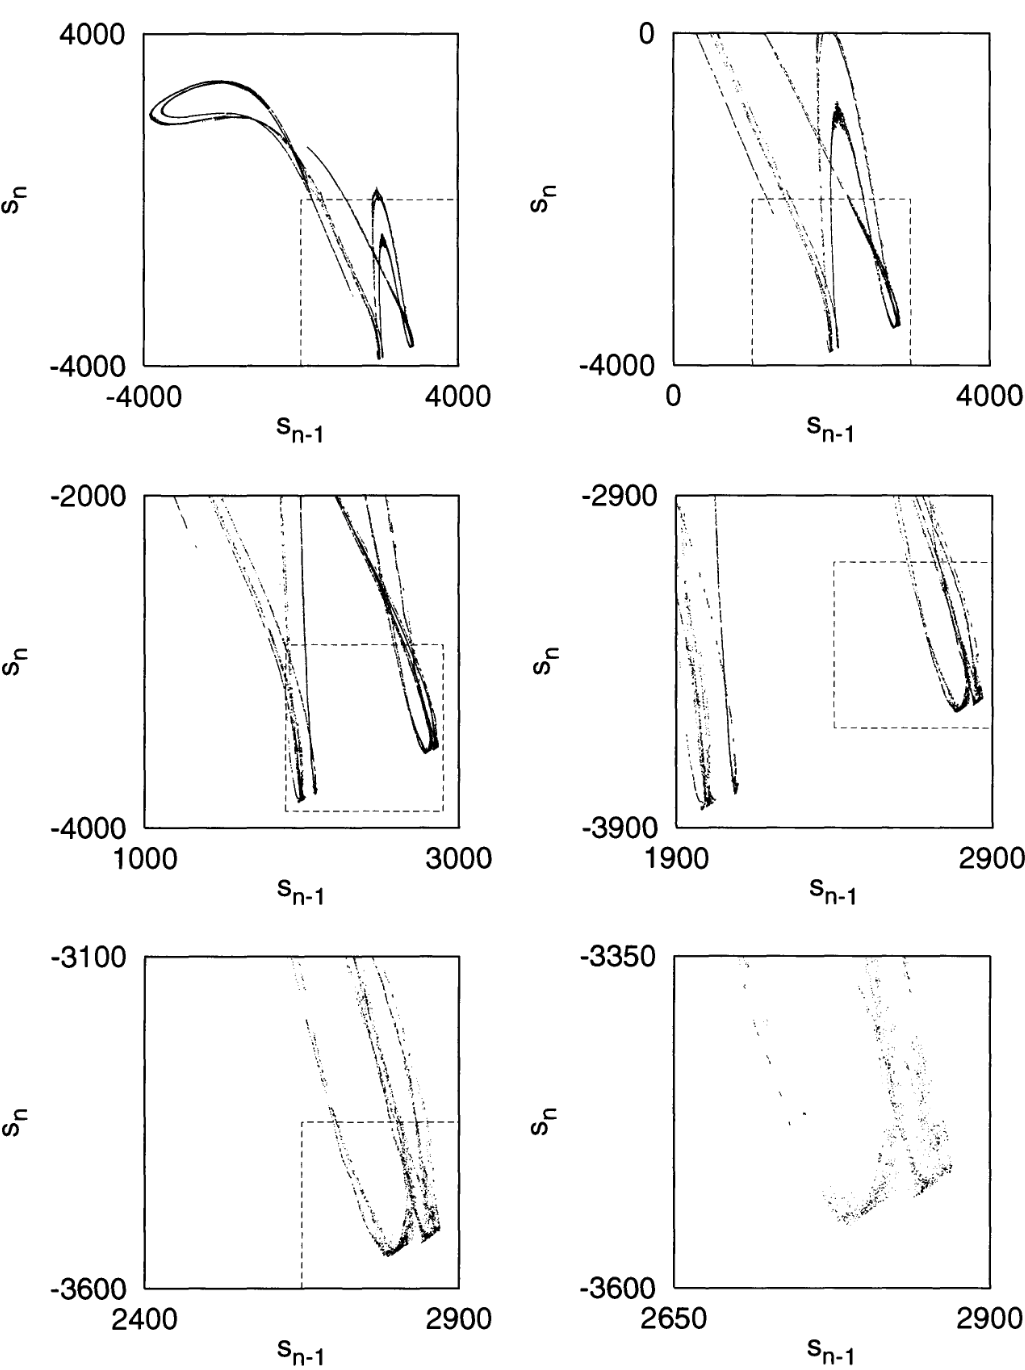
\includegraphics[width=0.8\textwidth]{Images/self-similarity.png}}
  \caption{Noise-reduced visualization of successive enlargements of highly self-similar attractor. (\cite{kantz2004})}
\label{fig:self-similarity}
\end{figure}

\section{State space reconstruction} \label{sec:state-space-reconstruction}
\subsection{Embedding} \label{sec:embedding}
In the previous section, we have introduced a concept of state space of a dynamical system. In the case of EEG analysis, however, our observations do not directly form a state space object, but a set of time series (a sequence of scalar measurements), one for each electrode. Moreover, it is necessary to deal with the fact that our data, however rich, rarely represent complete information about the studied system. In the case of EEG signals, the complete state of the system at any moment is determined by many variables, and the sensors are only able to collect traces of their cumulative effects (and noise). So we are confronted with a problem: how to convert this data into state space trajectories? This procedure is called \emph{state space reconstruction}.

% Broadly, one possible approach to non-linear time series analysis consists of the following steps: 
% \begin{enumerate}
%   \item reconstruction of the dynamics of given system from recorded data,
%   \item characterization of the reconstructed attractor,
%   \item checking validity of the results with surrogate data testing. \cite{stam2005}
% \end{enumerate}

To this goal, let $\mathbf{s}_n$ be the reconstructed vector we are trying to find, and let us have a time series of scalar measurements of a quantity depending on the current state of the system:
\begin{align} \label{eq:measurements}
  s_n = s(\mathbf{x}(n \Delta t)) + \eta_n \, ,
\end{align}
where $\mathbf{x}$ is a state space vector, $s(\cdot)$ is a measurement function and $\eta_n$ is a measurement noise. Furthermore, let us consider a function $\Phi: M \rightarrow \RR^m$, such that $\mathbf{s}_n = \Phi(\mathbf{x}(n \Delta t))$. Such function is called an \textbf{embedding}. In the following, we will discuss what properties does $\Phi$ have to satisfy so that it provides useful information about the true state space trajectories.

Before we do that, let us mention the following. As we have stated in Section \ref{sec:dynamical-systems}, our observations are formed by application of non-invertible measurement function $s: \RR^d \rightarrow \RR^{d'}$, $d' \ll d$, to the true states of the system. Aside from being a projection, $s$ may be also be a distortion. Therefore, it might seem impossible to reconstruct the true state space trajectory and this indeed may be the case in some situations. On the other hand, there are quantities invariant under distortion which may be preserved. \cite{andreas2000} Moreover, if our goal was to study only the attractor properties, perfect reconstruction may not even be desirable in the case that the attractor dimension is smaller than the dimension of the original space \cite{kantz2004}.

Firstly, note that we assume the studied dynamical system to be deterministic. If our reconstructed embedded space is to represent the true state space, evolution of any state on every trajectory we observe in the embedded space should depend only on its current state. Therefore, we may reasonably require $\Phi$ to be one-to-one, i.e. contain no intersections.

Secondly, since many of the attractor properties we care about (such as correlation dimensions, Lyapunov exponents, etc.) are only invariant under smooth non-singular transformations, in order to preserve these properties in the embedded space, we may require $\Phi$ to preserve the differential structure of $M$. This corresponds to the tangent space $D \Phi$ also being a one-to-one mapping. 

(TODO: Add images illustrating these two conditions.)

\subsection{The choice of embedding dimension}
In 1936, Whitney showed that every $n$-dimensional differentiable manifold can be embedded in $\RR^{2n+1}$, and that the set of such embeddings is open and dense in the space of smooth maps. \cite{thm:whitney} \footnote{The second part of the theorem is a consequence of the fact that two hyperplanes with dimensions $d_1$ and $d_2$ in $m$-dimensional space are likely to intersect if $d_1 + d_2 \geq m$.} This, in itself, is not necessarily useful in practice, since even dense sets can have measure zero. In 1991, Sauer was able to generalize Whitney's theorem as follows (in a simplified form):
\begin{thm}[Sauer, \cite{sauer1991}] \label{thm:sauer}
  Let $A$ be a compact fractal with box-counting dimension $d_A$, and let $A$ be a subset of a $m$-dimensional manifold. Then
  \begin{align*}
    \lbrace \Phi: A \rightarrow \RR^{d} | \Phi \in C^1, d > 2d_A \rbrace \text{ is an embedding with probability } 1.
  \end{align*}
\end{thm}

\subsection{Method of time delays}
There are two common approaches to the problem of state space reconstruction:
\begin{description}
  \item [Time delay embedding]: state space is reconstructed separately for each time series.
  \item [Spatial embedding]: each time series corresponds to a coordinate of the state space vector.
\end{description}

Time delay embedding was first proposed by N. H. Packard in 1980. Studying the Rossler system, Packard noticed that by sampling a single coordinate, he was able to obtain a faithful phase-space representation of the original system by simply using a value of a coordinate with its values at two previous times. \cite{packard1980} Indeed, since only a single sequence of scalar measurements is available, our only option for constructing the vectors $\mathbf{s}_n$ is by using values recorded at multiple different times. Packard's technique, however, can be useful in general.

In particular, for each time $t$, we define an embedding window $\tau_w$, and use measurements obtained at times $t'$ for $t-\tau_w \leq t' \leq t$. To this goal, we use $m$ measurements, $\tau$ elements apart. Here, $\tau$ is called \emph{lag} or \emph{time delay}, and is measured in units of sampling time. Using the notation of \ref{eq:measurements}, the time delay reconstruction is then formed by the following vectors:
\begin{align}
  \textbf{s}_n = (s_{n-(m-1)\tau}, s_{n-(m-2)\tau},\dots,s_{n-\tau}, s_n) \, ,
\end{align}
for $n > (m-1)\tau$. \cite{kantz2004} 

(TODO: add result from \cite{Kantz1997} either here or to experiments section about rising entropy with higher $\tau$. Deterministic behavior can be observed only when $\tau_w$ is smaller than the time scale of the foldings naturally produced as result of time embedding.)

A year after Packard's discovery, in \cite{takens1981}, F. Takens has proved theoretically that the attractor reconstructed using this method has the same dynamical properties (entropy, dimension, Lyapunov spectrum) as attractor of the original system.

Takens delay embedding theorem is an important result of non-linear time series analysis and can be stated as follows:
\begin{thm}[\cite{takens1981}] \label{thm:takens}
  Let $M$ be a compact\footnote{This theorem can be proved for $M$ non-compact provided less restrictions are imposed on $s$.} manifold specifying the state space of a deterministic dynamical system of dimension $n \in \NN$, $s : M \rightarrow \RR, s \in C^2$ a smooth measurement function, $f : M \rightarrow M, f \in C^2$ a smooth diffeomorphic state evolution function with a strange attractor of box-counting dimension $d_A$, and let $k > 2d_A$. Then the set of maps $\phi : M \rightarrow \RR^k$, defined by
  \begin{align}
    \phi(x) = (s(\mathbf{x}), s(f(\mathbf{x})), \dots, s(f^{k-1}(\mathbf{x}))),
  \end{align}
  for which $\Phi$ is an embedding is an open and dense set in the space of maps satisfying the assumptions above.
\end{thm}

Theorem \ref{thm:takens} ensures that when $m$ is chosen such that $m > 2d_A$, then the vector $\textbf{s}_n$ is a true embedding of the underlying attractor for almost any $\tau$ (note only sufficiency of the result). (TODO: How does this theorem relate to \ref{thm:sauer}? How does Sauer improve on it? Did I understand something wrong?)

\subsection{False nearest neighbors}

Of course, this method requires proper choice of parameters $m$ and $\tau$. From Theorem \ref{thm:takens} follows that vectors $\{\mathbf{s}_n\}$ are difeomorphic to the attractor $A$ of the system $M$ if $m$ is sufficiently large, specifically $m > 2d_A$ (note that $d_A$ may be much smaller than $\dim M$). On the other hand, $m$ adds redundancy, makes successive alogorithms less efficient. Moreover, the total time delay $m\tau$ is limited by the recording time. 

There are multiple methods of choosing the parameters. We will start with a description of an algorithm for determining the minimal sufficient embedding dimension $m$, known as \emph{false nearest neighbors} algorithm.
The false nearest neighbors algorithm is based on simple topological insight. If the embedding dimension $m$ is too small, some points that are close to each other in dimension $m+1$ (see Fig. \cite{}). Neighboring points satisfying this property are called \emph{false neighbors}.

(TODO: Mutual information algorithm for $\tau$)

\section{Non-linear measures}
\subsection{Lyapunov exponents}
Lyapunov exponents can be used to quantify sensitivity of a dynamical system to initial conditions. Consider a small sphere of similar initial conditions in the phase space of the attractor. As the the system evolves, this sphere expands at exponentially in all the $m$ directions at rates given by the spectrum of Lyapunov exponents. Hence, $m$ dimensional system has exactly $m$ Lyapunov exponents and the average rate of separation between two points in the phase space with similar initial conditions can be characterized by the largest Lyapunov exponent. A sigle positive exponents is a sufficient indication of chaos. 

In order to compute entire Lyapunov spectrum, it is necessary to measure the rate of separation along the appropriate Lyapunov directions. This requirement, however, is unnecessary for computation of only the Largest lyapunov exponent, as its direction dominates growth. Hence, the largest Lyapunov exponent $\lambda_1$ can be defined as

\begin{align}\label{eq:lyap}
  d(t) = C e^{\lambda_1 t}, 
\end{align}

where $d$ is a function of the average divergence, and $C$ is a factor normalizing for the initial separation.

\subsection{Correlation dimension}
Correlation dimension is a characteristic measure which describes complexity of the geometry of chaotic attractors.

Correlation sum $C(r)$ is defined as the fraction of points in the phase space whose distance is smaller than $r$:
\begin{align} \label{eq:corrsum}
  C(r) = \frac{2}{N(N-1)} \sum_{i<j} \Phi(r-\norm{\textbf{s}_i - \textbf{s}_j}).
\end{align}

If $C(r)$ decreases according to the power law with $r \rightarrow 0$ such that $C(r) \approx r^D$, then $D$ is called the correlation dimension, formally defined as

\begin{align} \label{eq:corrdim}
  CD = \lim_{r \rightarrow 0} \frac{\log C(r)}{r}.
\end{align}

\begin{figure} 
\centering
\noindent\makebox[\textwidth]{%
  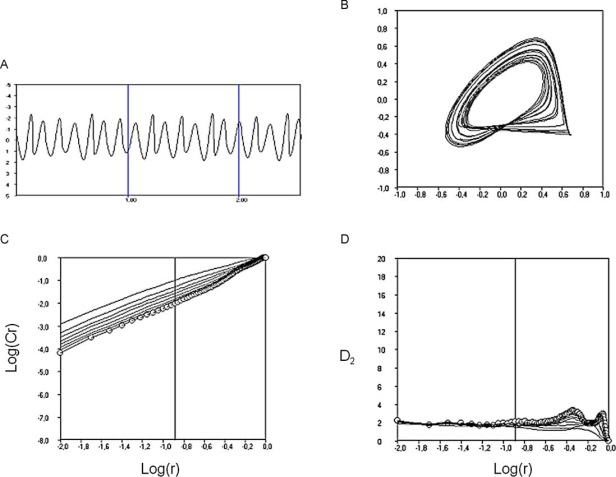
\includegraphics[width=0.8\textwidth]{Images/corrdim.png} }
  \caption{Computation of the correlation dimension \cite{stam2005}. TODO: Add description.}
\label{fig:corrdim}
\end{figure}

\section{Visual characterization of the dynamical system}
\subsection{Phase space plot}
\subsection{Poincare plot}
\subsection{Recurrence plot}
When presented with a task of finding regularities in seemingly chaotic data, one possible approach is analysing at least approximate repetitions of simple patterns, which can be further used for reconstruction of more complicated rules. Recurrence plot is a method of visualizing obtained state-space trajectory segments in relation to each other to achieve this goal. Furthermore, it can be used to test necessary conditions for validity of dynamical parameters derivable from a non-linear time series such as the information dimension, entropy, Lyapunov exponents, dimension spectrum, etc. The information contained in recurrence plots is not easily obtainable by other known methods. \cite{eckmann1987}

\begin{dfn}[\cite{eckmann1987}]
  Let $N$ be the length of given time series, $\mathbf{s}_i$ for $i \in \{1,2,\dots,N \}$ be a $i$-th delay vector of any integer embedding dimension, $\norm{\cdot}$ a norm, $\Theta(\cdot)$ a Heaviside step function, and $\epsilon \in \RR_0^+$ a tolerance parameter. Then, \textbf{recurrence plot} is the matrix
  \begin{align}
    M_{ij} = \Theta(\epsilon - \norm{ \textbf{s}_i - \textbf{s}_j }) \, .
  \end{align}
\end{dfn}

In other words, $M_{ij}$ is a symmetric\footnote{Although this is true for our definition, it may not be true for an alternative definition using a more general topology instead of a norm.} binary $N x N$ matrix, where $M_{ij} = 1$ when $i$-th and $j$-th points of the reconstructed trajectory enter each other's $\epsilon$ neighborhood.

The essential drawback of recurrence plot is their size - it is quadratic in the length of the time series. A simple way of reducing its dimension is to partition the time series into disjoined segments, and let $M_{ij}$ represent the distance between those two segments. This is known as \textbf{meta-recurrence plot}. \cite{kantz2004} (TODO: Find a justification for using them.)

(TODO: Cross-recurrence plots may be useful? Only between two series. Joint recurrence plots may be used to detect phase synchronization.)

\section{Applications in disease diagnosis}\label{sec:applications}
Although non-linear dynamical analysis of EEG signal has been successfully applied to many psychological and psychiatric conditions, such as insomnia, schizophrenia, epilepsy, dementia, Alzheimer's disease, the number of studies applying methods of non-linear time series analysis for clinical depression diagnosis is relatively limited. \cite{rodriguez2015}

It has been found that the EEG dynamics of depressed patients exhibit more predictability than those of non-depressed ones, with this indicator receding after treatment. \cite{nandrino1994} \cite{pezard1996}

Another study analyzed sleep EEGs of depressed and control subjects, and found significantly decreased values of Lyapunov exponents in a sleep stage IV in depressed relative to control. \cite{roschke1995}

In 2012, Ahmadlou et al. decomposed 5 EEG channels recorded from frontal lobes of healthy and depressed patients using wavelet filter banks, measured their complexity using Higuchi's fractal dimension, subsequently used ANOVA to discover the most meaningful differences between the groups, and trained a probabilistic neural network classifier, achieving 91.3\% classification accuracy on limited amount of data. This research suggested potential of frontal lobe signal assymetry as a measure for depression. \cite{ahmadlou2012}

In the same year, Hosseinifard et al. extracted Higuchi's correlation dimension, Lyapunov exponents and Higuchi's fractal dimension from 4 EEG channels of 90 patients split evenly between depressed and non-depressed subjects, achieving 90\% accuracy using a logistic regression classifier. \cite{hosseinifard2013}

In 2013, Bachmann et al. compared two non-linear analysis methods, spectral assymetry index (SASI) and Higuchi's fractal dimension (HFD), for depression diagnosis, on 34 subjects split evenly between depressed and control group. SASI achieved true detection rate in 88\% in depressives and 82\% in the controls, while HFD provided true detection rate of 94\% in the depressives and 76\% in the controls. \cite{bachmann2013}

Sleep disorder diagnosis may also relevant to this work for the very close connection of depression with disturbed sleep and insomnia \cite{nutt2008}. The first study emplying techniques of non-linear analysis on human EEG was published in 1985 and dealt with sleep recordings. \cite{babloyantz1985} This early success sparked intensive research focus on applying non-linear analysis to sleep data, thus generating relatively large amount of results. 

Many studies focused of extracting Lyapunov exponents of EEGs measured during various sleep stages. The general pattern that emerged was that deep sleep stages exhibit lower complexity evidenced by lower dimensionality lower values of the largest Lyapunov exponent \cite{stam2005}.

\chapter{Convolutional Neural Networks}

\section{Mathematical background}
TODO: Do we really need this section???

\begin{dfn}
  Let $I$ be an image function, $K$ a kernel. A (discrete) \textbf{convolution} of $I$ and $K$ is a functional defined as
  \begin{align}
    (I*K)(i,j) = \sum_m \sum_n I(m,n) K(i-m, j-n) \, .
  \end{align}
\end{dfn}

Note that some machine learning libraries (such as Tensorflow) implement \textbf{cross-correlation} instead of convolution, but preserving the term convolution for the operation. Cross-correlation corresponds to convolution with kernel rotated by 90 degrees:
\begin{align}
  (I*K)(i,j) = \sum_m \sum_n I(m,n) K(i+m, j+n) \, .
\end{align}
Unlike convolution, cross-correlation is not commutative, but this property is not required for neural network applications.

\begin{dfn}
  Let $f$ be arbitrary function, and $\mathcal{D}$ its degradation operator. We say $f$ is \textbf{invariant} under $\mathcal{D}$ if
  \begin{align}
    \mathcal{D}(f) \equiv f \, .
  \end{align}
\end{dfn}

For the following, the reader needs to understand the term \textbf{equivariance}. 
\begin{dfn}[\cite{pitts2013}]
  Let $G$ be a group and $X$, $Y$ its G-sets. Then $F:X \rightarrow Y$ is called an \textbf{equivariant function} if
  \begin{align}
    F(g(x)) = g(F(x))
  \end{align}
  for all $G$ actions $g$ and $x \in X$.
\end{dfn}

For our purposes, we can view $G$ as a group of transformations, and then equivariance as a commutative property of a function with regards to the transformations. In other words, computing the function and then applying the transformation has the same effect as applying the transformation and then computing the function.

TODO: This is probably too basic to be here

\textbf{Gradient descent} is a first order iterative method of finding an extremum a differentiable function $f : \RR \rightarrow \RR^n$, $f \in C^1$, based on continually moving a point in its domain in the direction of negative of its gradient at that point, until the absolute value of the gradient (or the step size) is below a certain threshold. See Algorithm \ref{alg:gd}.

\begin{algorithm}
  \caption{Gradient descent algorithm.}
  \label{alg:gd}
\begin{algorithmic}[1]
  \State Initialize random $x_0 \in D(f)$
  \State $n \gets 0$
  \State step\_size $\gets 1$  
  \While{step\_size $ < \text{threshold}$ and $n < $ iters\_limit}
  \State $x_{n+1} = x_n - \epsilon \nabla_{x_n} f$
  \State step\_size $\gets |x_{n+1} - x_n|$ 
  \State $n \gets n + 1$
  \EndWhile
\end{algorithmic}
\end{algorithm}

\textbf{Stochastic gradient descent}\dots

\section{History}

The classical approach to image pattern recognition consists of the following stages:
\begin{description}
  \item[preprocessing:] supressing unwanted distortions and noise, enhancement beneficient for further processing,
  \item[object segmetation:] separating disparate objects from the background,
  \item[feature extraction:] gathering relevant information about the properties of the objects, removing irrelevant variations,
  \item[classification:] categorizing segmented objects based on obtained features into classes.
\end{description}

The preprocessing step may require additional assumptions about the data or further processing, which are potentially too restrictive or too broad. Getting around this limitation requires dealing with complications such as high dimensionality of the input (number of pixels) and desirability of invariance towards a number of allowable distortions and geometrical transformations.

Artificial neural networks in combination with gradient-based learning are one possible solution to the problem. By gradually optimizing a set of weights based on a training data set using a differentiable error function, they provide a framework for learning a suitable set of assumptions automatically from the data.

One of the oldest neural network architectures, fully connected multi-layer perceptron (FC-MLP), can be used for image pattern recognition. However, it has the following drawbacks:
\begin{description}
  \item[parameter explosion:] the number of parameters of such network is exponential in the number of layers, increasing the capacity of the network and therefore need for more data,
  \item[no invariance:] no invariance even with respect to common geometrical transformation such as translation, rotation and scaling,
  \item[ignoring input topology:] natural images exhibit strong local structure and high correlation between intensities of neighboring pixels, but FC-MLPs are unstructed - inputs can be presented in any order.
\end{description}

Although the main idea dates back 1980 with K. Fukushima's neocognitron \cite{fukushima1982}, the back-propagation algorithm was not known at the time. The first convolutional architecture successfuly applied on an image pattern recognition problem by attempting to solve the aforementioned problems, dubbed LeNet-5, was proposed in 1998 by Y. LeCun, L. Bottou, Y. Bengio and P. Haffner \cite{LeCun1998}.

\section{Description}

\begin{figure} 
\centering
\noindent\makebox[\textwidth]{%
  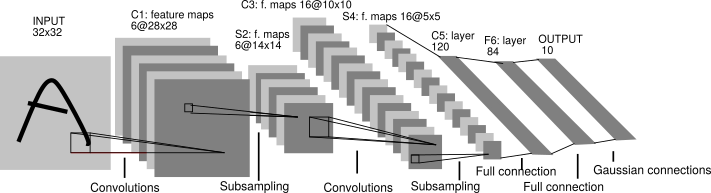
\includegraphics[width=0.8\textwidth]{Images/lenet-5.png} }
  \caption{LeNet-5 architecture \cite{lecun1999}.}
\label{fig:lenet-5}
\end{figure}

Bearing resemblence to visual processing in biological organisms \footnote{As early as in 1968, D. H. Hubel and T.N. Wiesel discovered that some cells (called simple cells) in cat's primary visual cortex (V1) with small receptive fields (shared by neighboring neurons) are sensitive to straight lines and edges of light of particular orientation, and other cells (called complex cells) with larger receptive fields further in the visual cortex also respond to straight lines and edges, but with invariance to translation \cite{Hubel1968}.}, LeNet-5 proposed the following design principles to enforce \emph{shift, scale and distortion invariance}: \cite{lecun1999}
\begin{description}
  \item[local receptive fields:] each neuron in a layer receives input from a small neighborhood in the previous layer,
  \item[shared weights:] each layer is composed of neurons organized in planes within which each neuron have the same weight vector (feature map),
  \item[spatial subsampling:] adding a subsampling layers, which reduce the resolution of the previous layer by averaging or taking the maximal value of neighboring pixels in the previous layer.
\end{description}

\subsection{Local receptive fields}
\emph{Local receptive fields} enable the network to synthesize filters that produce strong response to elementary salient features in the early layers (such as lines, edges and corners in a visual input, and their equivalents in other modalities), and then learn to combine them in the subsequent layers to produce higher-order feature detectors.

\begin{figure} 
\centering
\noindent\makebox[\textwidth]{%
  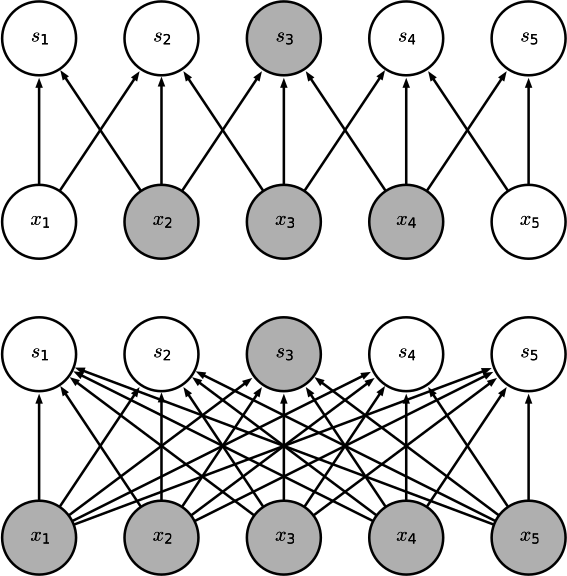
\includegraphics[width=0.5\textwidth]{Images/receptive_field.png} }
  \caption{Receptive field. \cite{goodfellow2016}}
\label{fig:receptive_field}
\end{figure}

For a visual explanation of the concept of receptive field, see Figure \ref{fig:receptive_field}. The locality of of those receptive fields implies sparser connectivity, and hence more efficient computations in comparison with fully connected neural networks. A fully connected neural network with no hidden layers with $m$ inputs and $n$ outputs has $m \times n$ weight parameters, and the correspoding feed forward pass (matrix multiplication) is of $O(m \times n)$ time complexity per input. If the number of connections per output unit is limited to $k < m$, the achieved runtime is $O(k \times n)$, where $k$ is usally in practice several orders of magintude smaller than $m$. \cite{goodfellow2016}

In shallow neural networks, locality of receptive fields implies locality of ``influence'' of each input unit on the output. In deep neural networks, on the other hand, units in the deeper layers can be indirectly connected to some or all units of the input, thus enabling them to achieve aforementioned effect of combining more complex features from simpler ones.

\subsection{Shared weights}
With \emph{shared weights}, neural units in a layer with differing receptive fields have the same feature map and the same feature detecting operation (convolution with feature map kernel followed by additive bias and a application of a non-linear function) is performed on differing parts of the image (see Figure \ref{fig:shared_weights}). A single convolutional layer is composed of multiple feature detecting planes.

Shared weights principle exploits the fact that in natural images, a function of small number of neighboring pixels can be useful in multiple parts of the image. For example, an edge detector can be used accross the entire image to detect edges in the first layer, an object detector can then be used to detect presence of edges in particular arrangements in the next layer, etc.

Although it does not reduce the time complexity of the feedforward pass, it does reduce the memory requirements. If the kernel size is $k$, $m$ the number of inputs, $n$ the number of outputs, the number of parameters per layer is $k$ instead of $m \times n$ (per feature detecting plane) in a fully connected case. Since $k$ is usually in practice several orders of magnitude smaller than $m$, and usually $m$ and $n$ are comparable in size, the memory savings are highly significant. \cite{goodfellow2016}

One of the drawbacks of classical CNNs is that although convolution in combination with weight sharing causes layer output to be equivariant to translation of the input, this is not the case for scaling and rotation. Moreover, equivariance to input may not be always desirable. Consider a case of face detection, where all training and test images are centered. Then, the relative positions of individual features are important, and it may be favorable to fix feature detectors (and thus weights) to certain locations in the image.

\subsection{Pooling}
\begin{figure} 

\centering
\noindent\makebox[\textwidth]{%
  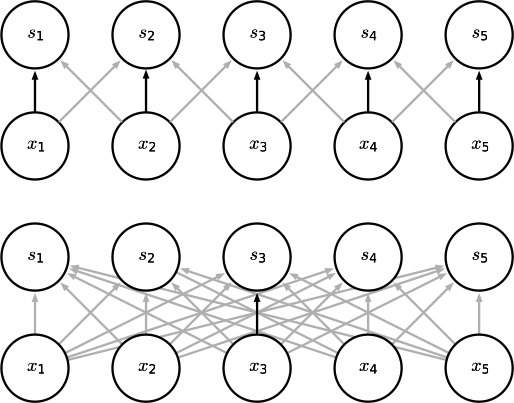
\includegraphics[width=0.5\textwidth]{Images/shared_weights.png} }
  \caption{Shared weights. \cite{goodfellow2016}}
\label{fig:shared_weights}
\end{figure}

The final output activations of a convolutional layer are computed in subsequent stages:
\begin{enumerate}
  \item linear unit activations are computed via the convolution operation,
  \item a non-linear activation function is applied to the activations,
  \item a spatial subsampling (pooling) operation is applied.
\end{enumerate}

The rationale behind applying a non-linearity is it makes the network capable of modelling non-linear functions. Common activation functions include rectified linear $\max(0,x)$, sigmoid $\frac{1}{1+\exp(-x)}$, hyperbolic tangent $\tanh$, and many others. They have varying properties making them useful in different situations. We will not explore them further here.

\emph{Pooling} operation splits the neural units into sets of multiple adjacent activations and computes a summary statistic, such as the maximum element (max pooling) or the average (average pooling), per such set and outputs the result. If the stride between the sets is greater than one, the spatial dimension of output is decreased relative to input (subsampling).

The purpose of spatial subsampling is to ensure scale and distortion invariance\footnote{Whether it achieves this goal has been famously doubted by Geoffrey Hinton: ``The pooling operation used in convolutional neural networks is a big mistake and the fact that it works so well is a disaster.'' \cite{}} by reducing the precision at which a feature is encoded in a feature map by reducing its resolution - when scale and distortion invariance is assumed, the exact location of a feature becomes less important and is allowed to exhibit slight positional variance - roughly speaking, an ``approximate'' translation invariance.

Although the combination of convolution and pooling performs well in many practical situations, it has multiple drawbacks. For example, the learned representations are not rotation invariant and thus, to mitigate this, the capacity of the network has to be increased and the training dataset must be enhanced to contain examples of rotated features, often extending the amount of data necessary and training time. A number of alternative approaches were suggested in the litarature.\footnote{For instance, Hinton's \emph{CapsNet}, described e.g. in \cite{sabour2017}, is an attempt to transform the manifold of images of similar shape (which is highly non-linear in the space of pixel intensities) to a space where it is globally linear by the way of using so called capsules instead of traditional convolutional layers.} For another example of a limitation, see Figure \ref{fig:drawbacks}.

\begin{figure} 
\centering
\noindent\makebox[\textwidth]{%
  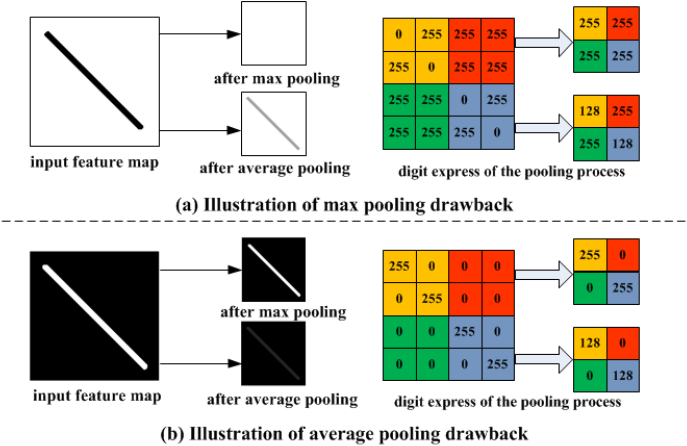
\includegraphics[width=0.8\textwidth]{Images/drawbacks.png} }
  \caption{Examples of drawbacks of the pooling operation. Max pooling discards all except the maximum element, and valuable information may thus be lost. Average pooling considers all the values, and the information about their contrast is reduced. Moreover, extreme values may have undesired effects on the result. \cite{yu2014}}
\label{fig:drawbacks}
\end{figure}


\section{Applications}
Maybe mention an example of how LeNet-5 was improved on subsequently (AlexNet, ResNet, etc.)? But this changes all the time\dots

\section{CapsNets?} \label{sec:capsnets}
Does it make sense trying them? I found a only a few successful implementations. Maybe it would be better to try those after we have some results already, because it seems risky - we might end up with nothing.

\chapter{Experiments}

\section{Dataset}
The EEG recordings were performed by and obtained from the Czech National Institute of Mental Health. The dataset comprises total of 133 subjects, 104 women and 29 men, ranging in age from 30 to 65 (47.7 $\pm$ 9.58). Geriatric Depession Scale questionnaire assessed by a trained psychologist was used to measure depression severity. This psychometric measurement results in a depression score ranging from 0 (normal) to 40 (severe depression). 

The experiment lasted 4 weeks. At the beginning of week 1, each subject's depression score was measured, their EEG signal was recorded, and, based on the measurement and patient's history, prescription of up to 4 drugs was made. After 4 weeks, depression score was remeasured and EEG signal recorded again.

During the EEG recording, 19 electrodes were placed on the scalp in accordance with the Internation 10-20 system (FP1, FP2, F3, F4, C3, C4, P3, P4, O1, O2, F7, F8, T3, T4, T5, T6, Fz, Cz, Pz). 99 subjects EEG signal was measured at sampling frequency $f_s$ of 250 Hz, while 1000 Hz was used for the remaining 34 patients. The patients were not told to close their eyes for the duration of the recording, resulting in unwanted artifacts in the signal. Some of the artifacts were removed manually by the researchers by omitting those parts from the recording, and concatenating the remaining parts. Durations of the resulting measurements range from 23.5 s to 170 s (75.6 $\pm$ 20 s) for $f_s = 250$ Hz , and from 48.8 s to 140.4 s (79.5 $\pm$ 18.4 s) for $f_s = 1000$ Hz.

\section{Preprocessing}
Recordings of insufficient duration were not used for further analysis. The threshold was selected to be 60 s, resulting in exclusion of 26 recordings from the total of 266.

All signals were highpass filtered with 0.5 Hz frequency and lowpass filtered with 70 Hz frequency. Our hypothesis is that such filter should not affect signals of our interest, since neural oscillations are known to lie inside the unmodified frequency band.
  
Lastly, recordings of $f_s = 1000$ Hz were downsampled to $250$ Hz using the Fourier method.

\section{Feature extraction}
Based on multiple studies successfully applying non-linear dynamical analysis on the problem of psychological disorder diagnosis mentioned in Section \ref{sec:applications}, we decided to extract the following non-linear features, quantifying the amount chaos and complexity of the signal.

In the first experiment, we used time-delay embedding (see Section \ref{sec:embedding}), resulting in 5 x 19 features for each measurement.  

\subsection{Largest Lyapunov exponent}
Largest Lyapunov exponent (LLE) was computed using the Rosenstein's algorithm \cite{Rosenstein1993}. This algorithm was found to be robust to noise and the choice of lag and embedding dimension.

First, it reconstructs phase space trajectory using the method of delays described in Section \ref{sec:embedding}. The lag is selected as the value for which the autocorrelation function drops to below $1-1/e$ of its initial value. Then, for each point on the reconstructed trajectory $\textbf{s}_n$, a nearest neighbor $\textbf{s}_{\hat{n}}$ is found as
\begin{align*}
  d_n(0) = \min_{\hat{n} \neq n}{\norm{\textbf{s}_n - \textbf{s}_{\hat{n}}}}, 
\end{align*}

where, additionaly, the nearest neighbors have temporal separation greater then the reciprocal of the mean frequency of the power spectrum of the time series, so that they can be safely considered to be nearby initial conditions for different trajectories (this separation, however, is restricted to be at most $1/4$ of the time series length). The mean rate of separation between the nearest neighbors is then an unbiased estimator for the LLE (TODO: Find citation for this claim.)

From the definition of the LLE \ref{eq:lyap}, the algorithm proceeds by assuming that each pair of nearest neighbors diverge approximately at the rate given by the LLE:

\begin{align*}
  d_n(i) \approx d_n(0)e^{\lambda_1 n \Delta t}. 
\end{align*}

By taking the logarithm of both sides,

\begin{align*}
  \ln d_n(i) \approx \ln d_n(0) + \lambda_1 n \Delta t, 
\end{align*}

we obtain a set of lines (one for each index $n$), whose slope is an approximation of the largest Lyapunov exponent. Hence, the value of $\lambda_1$ is approximated as the slope of least squares fitted line through the mean log divergence $\overline{d}$,

\begin{align*}
  \overline{d}(i) = \langle \ln d_n (i) \rangle.
\end{align*}

\subsection{Correlation dimension}
The simplest version of the Grassberger-Procaccia algorithm was used to compute the correlation dimension. \cite{grassberger1983} The value of the correlation integral $C(r)$ from the definition \ref{eq:corrsum} is computed for multiple values of $r$ in range from $0.1*\sigma$ to $0.5*\sigma$, where $\sigma$ is the standard deviation of the time series, and a least squares straight line is plotted through the plot of $\ln C(r)$ against $\ln r$. Correlation dimension is approximated as the slope of the line.

\subsection{Sample entropy}
\subsection{Detrended fluctuation analysis}
\subsection{Hurst exponent}

\section{Unsupervised analysis of before / after treatment differences}
As the first step of our analysis, we conducted an investigation of the differences in the non-linear measures computed from the signals obtained before and after treatment.

To this goal, we started by simply plotting each measure's mean value over channels for the recording before and after administration of drugs for all patients. Moreover, we performed two-sided Kolmogorov-Smirnov test for the null hypothesis that the distributions of values computed for measurements before and after treatment are the same.

We found that for each measure except correlation dimension, its average over channels, although differring between subjects, is remarkably stable for all patients accross measurements. This means that except for correlation dimension, information about any change between measurements was not caputered by the computed non-linear measures (see Figure \ref{fig:lyap_all}, \ref{fig:corrdim_all}).

Moreover, we found that for all measures, either for mean value or all channels, we cannot reject the hypothesis that the computed values are drawn from the same distribution. This is true even when patients responding and not responding to treatment are considered separately.

Apart from computing the mean, principal component analysis was used to reduce the number of dimensions of the 19 dimensional feature vectors. By visually inspecting projections into 2, 3 (2/3D plot)  and 4 dimensions (a heatmap), we were unable to find any separation boundary between before and after group. \footnote{And neither for male / female, responding / non-responding, age < 40 / age > 50 groups, and in groups based on depression scores.} (see Figure \ref{fig:pca2d}, \ref{fig:pca3d}, \ref{fig:heatmap}).

Also, by looking at the subjects above 90th percentile of euclidean distance between before and after vectors in the projected space, we were unable to find any regularity. Subjects in those groups seem to be drawn randomly from the dataset.

\begin{figure} 
\centering
\noindent\makebox[\textwidth]{%
  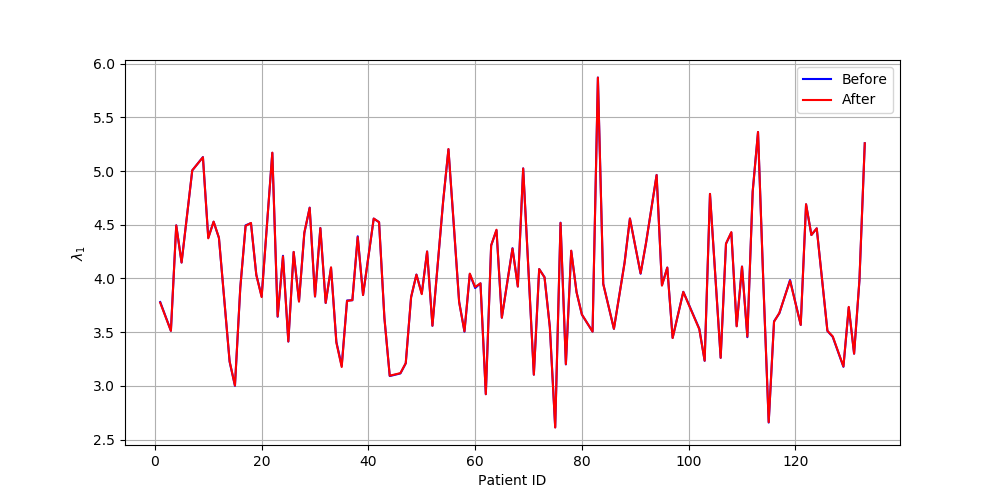
\includegraphics[width=0.8\textwidth]{Images/lyap_all.png} }
  \caption{}
\label{fig:lyap_all}
\end{figure}

\begin{figure} 
\centering
\noindent\makebox[\textwidth]{%
  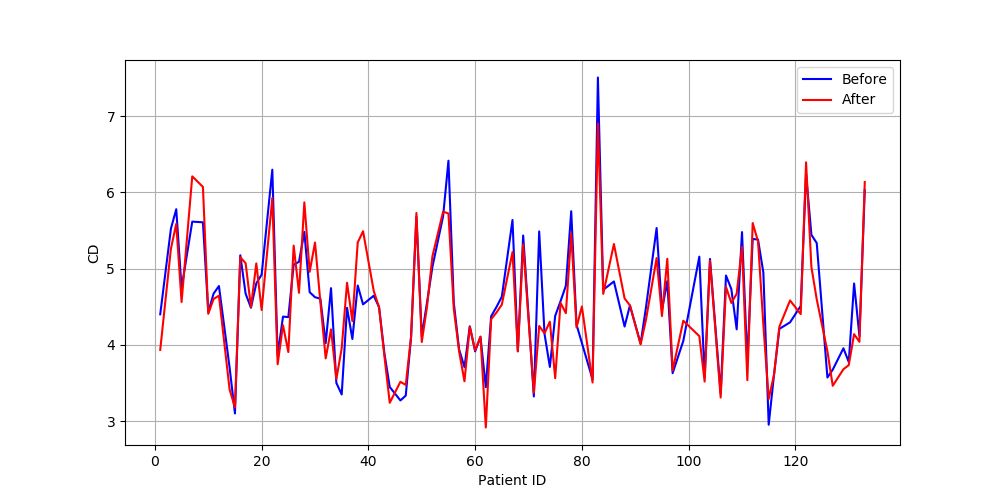
\includegraphics[width=0.8\textwidth]{Images/corrdim_all.png} }
  \caption{}
\label{fig:corrdim_all}
\end{figure}

\begin{figure} 
\centering
\noindent\makebox[\textwidth]{%
  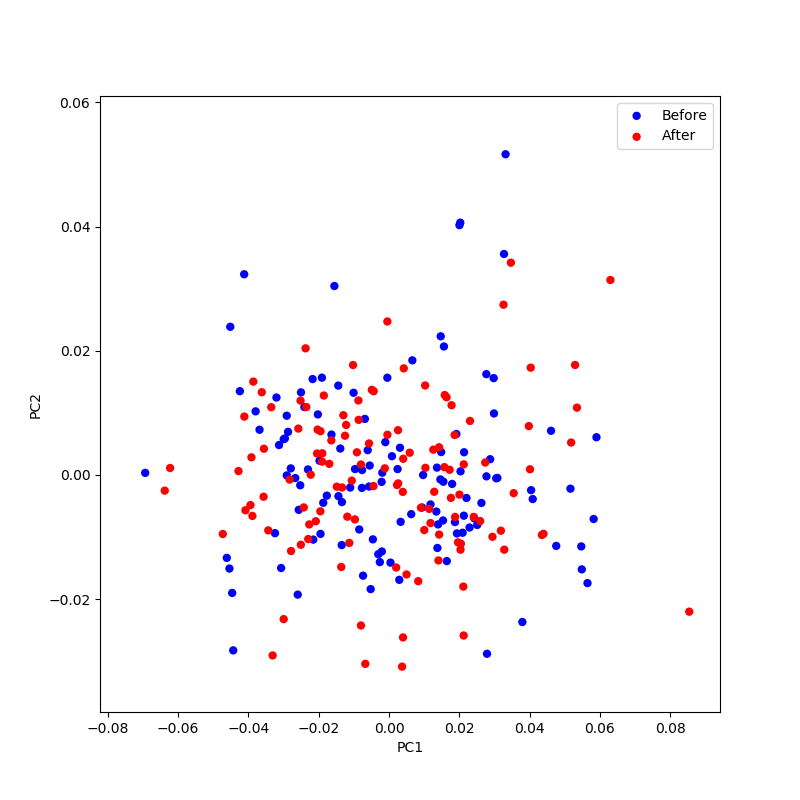
\includegraphics[width=0.8\textwidth]{Images/pca2d.png} }
  \caption{}
\label{fig:pca2d}
\end{figure}

\begin{figure} 
\centering
\noindent\makebox[\textwidth]{%
  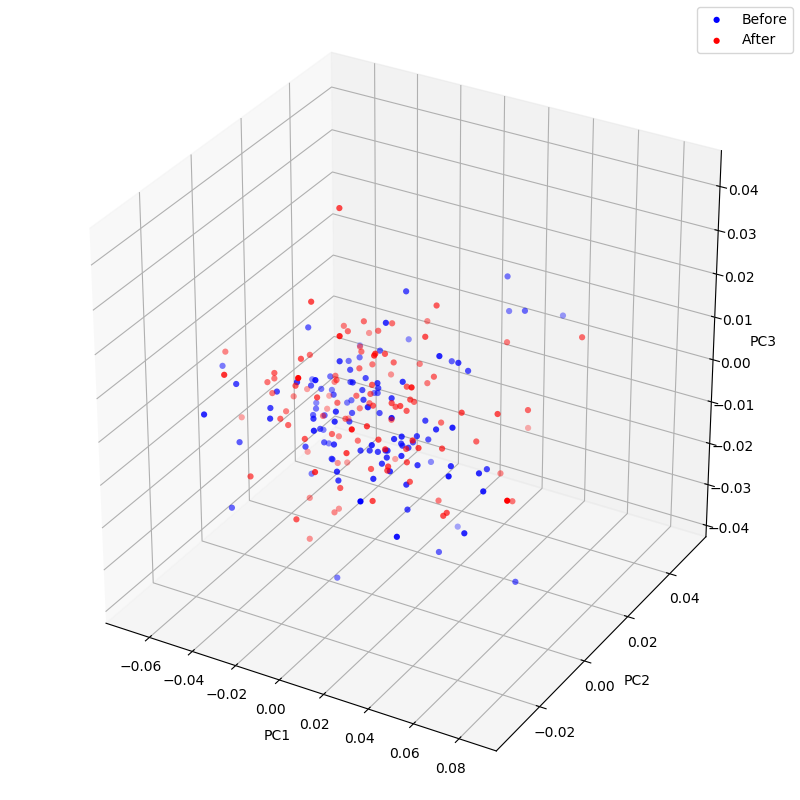
\includegraphics[width=0.8\textwidth]{Images/pca3d.png} }
  \caption{}
\label{fig:pca3d}
\end{figure}

\begin{figure} 
\centering
\noindent\makebox[\textwidth]{%
  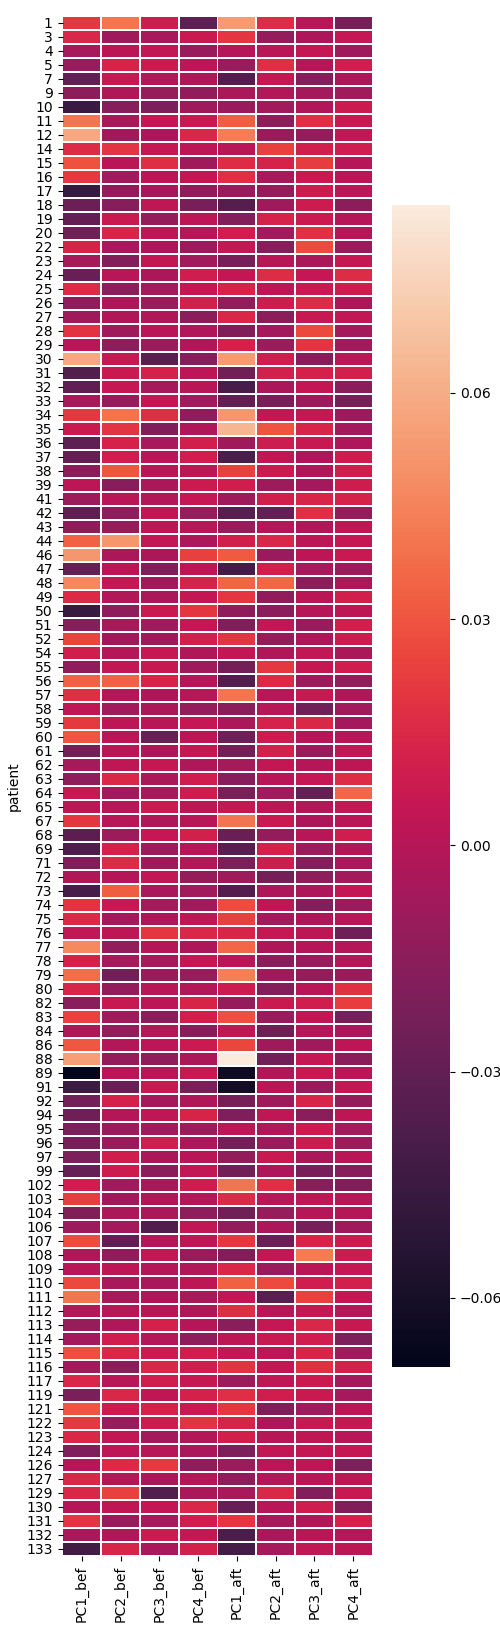
\includegraphics[width=0.4\textwidth]{Images/heatmap.png} }
  \caption{}
\label{fig:heatmap}
\end{figure}
\section{Results}

\chapter*{Conclusion}

\bibliographystyle{plain}
\bibliography{refs}
\end{document}
